\subsection{Temporal Difference Learning for Model Predictive Control}

\subsubsection{Configuration}
Our TDMPC agent uses a hidden size of 256 neurons for all linear layers, a latent dimension of 50, a 5-step planning horizon, 512 trajectory samples, a 0.05 mixture coefficient, an initial temperature of 0.5 (decaying by 0.001 to a minimum of 0.1), a reward weight of 0.1, and a discount factor ($\gamma$) of 0.99. All networks—encoder, dynamics, reward, actor, and value—consist of two linear layers, each followed by ReLU activations. The learning rate parameters were calibrated at $10^{-3}$ for the world model, $10^{-4}$ for the actor, and $10^{-3}$ for the value function.

\paragraph{Pendulum-v1}
To verify that our implementation of the TDMPC agent was functioning correctly, we trained our agent for 250 episodes in the Pendulum-v1 environment. We observed the agent successfully solve the relatively simple environment around the 150-th episode mark.

\paragraph{Hockey-Env}
We conducted our training over 2,000 episodes against the provided BasicOpponent-weak benchmark. 
As illustrated in Figure \ref{fig:rewards_tdmpc}, our agent's learning journey reveals a clear progression. In the initial phases, the agent had yet to learn a good representation of the world, resulting in mostly losses against the opponent. However, at approximately the 1,000-episode mark we can already see the agent winning nearly 50\% of the games. A significant performance leap occurred around episode 1,750, suggesting the development of better defensive and offensive strategies against the very formulaic bot.
\begin{figure}[htbp]
    \centering
    \subfloat[Smoothed reward over the training episodes]{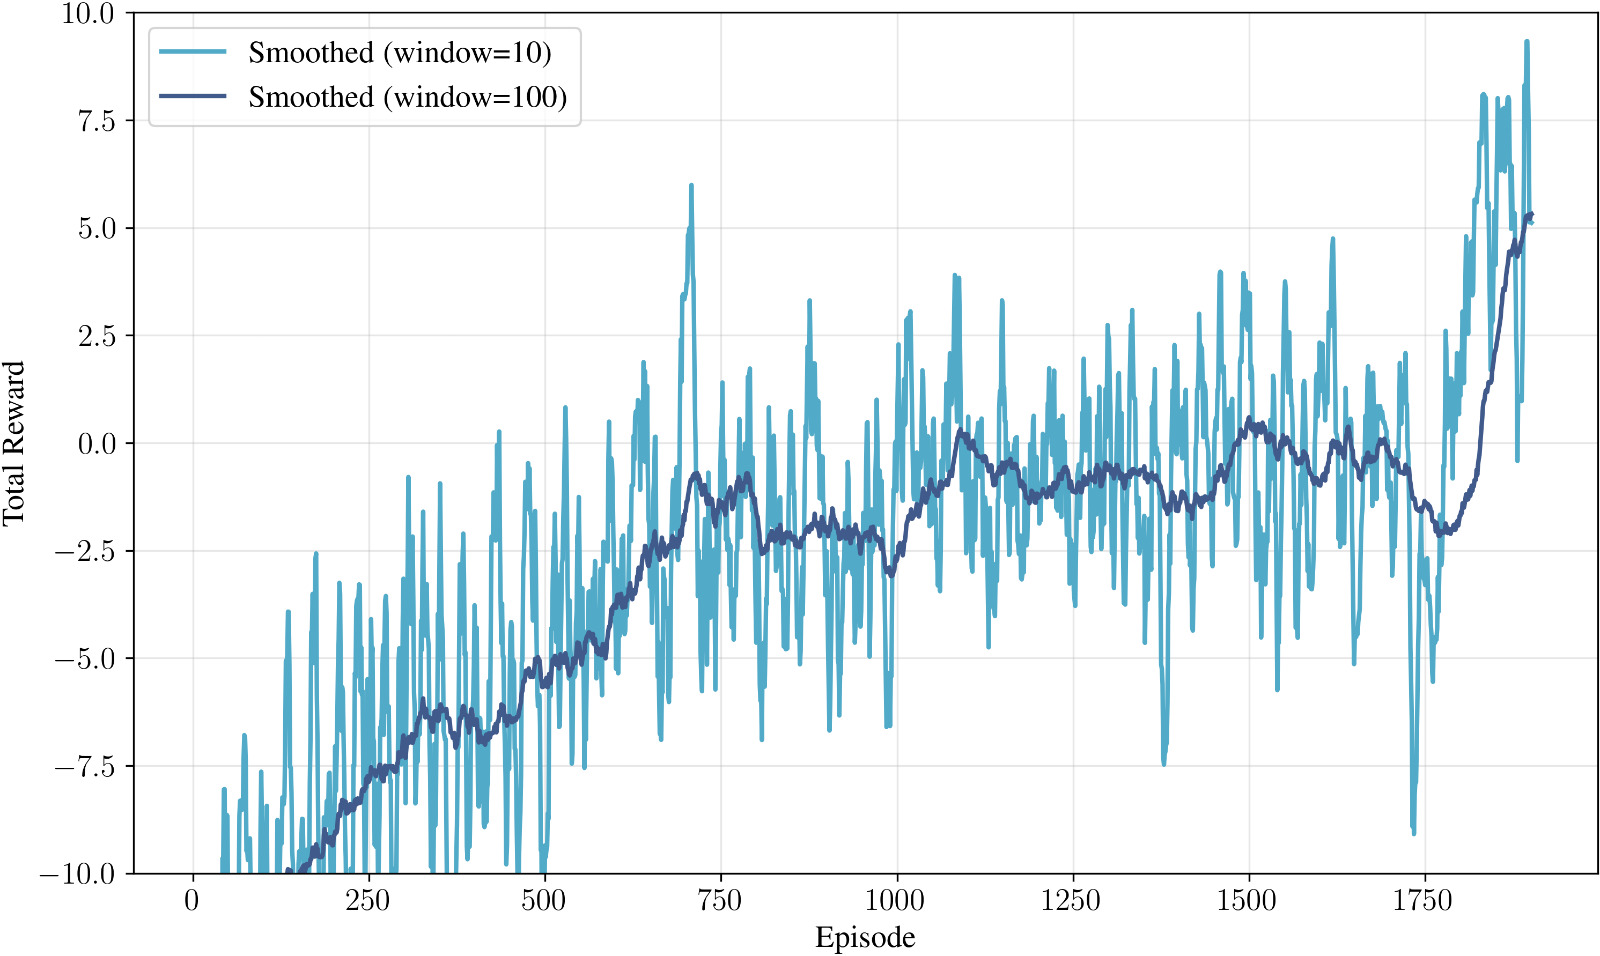
\includegraphics[width=0.5\textwidth]{Plots/episode_rewards_tdmpc.jpeg}\label{fig:rewards_tdmpc}}
    \hspace{0.5cm} % Adds horizontal space between the two images
    \subfloat[Winrate vs BasicOpponent-weak across 250 matches]{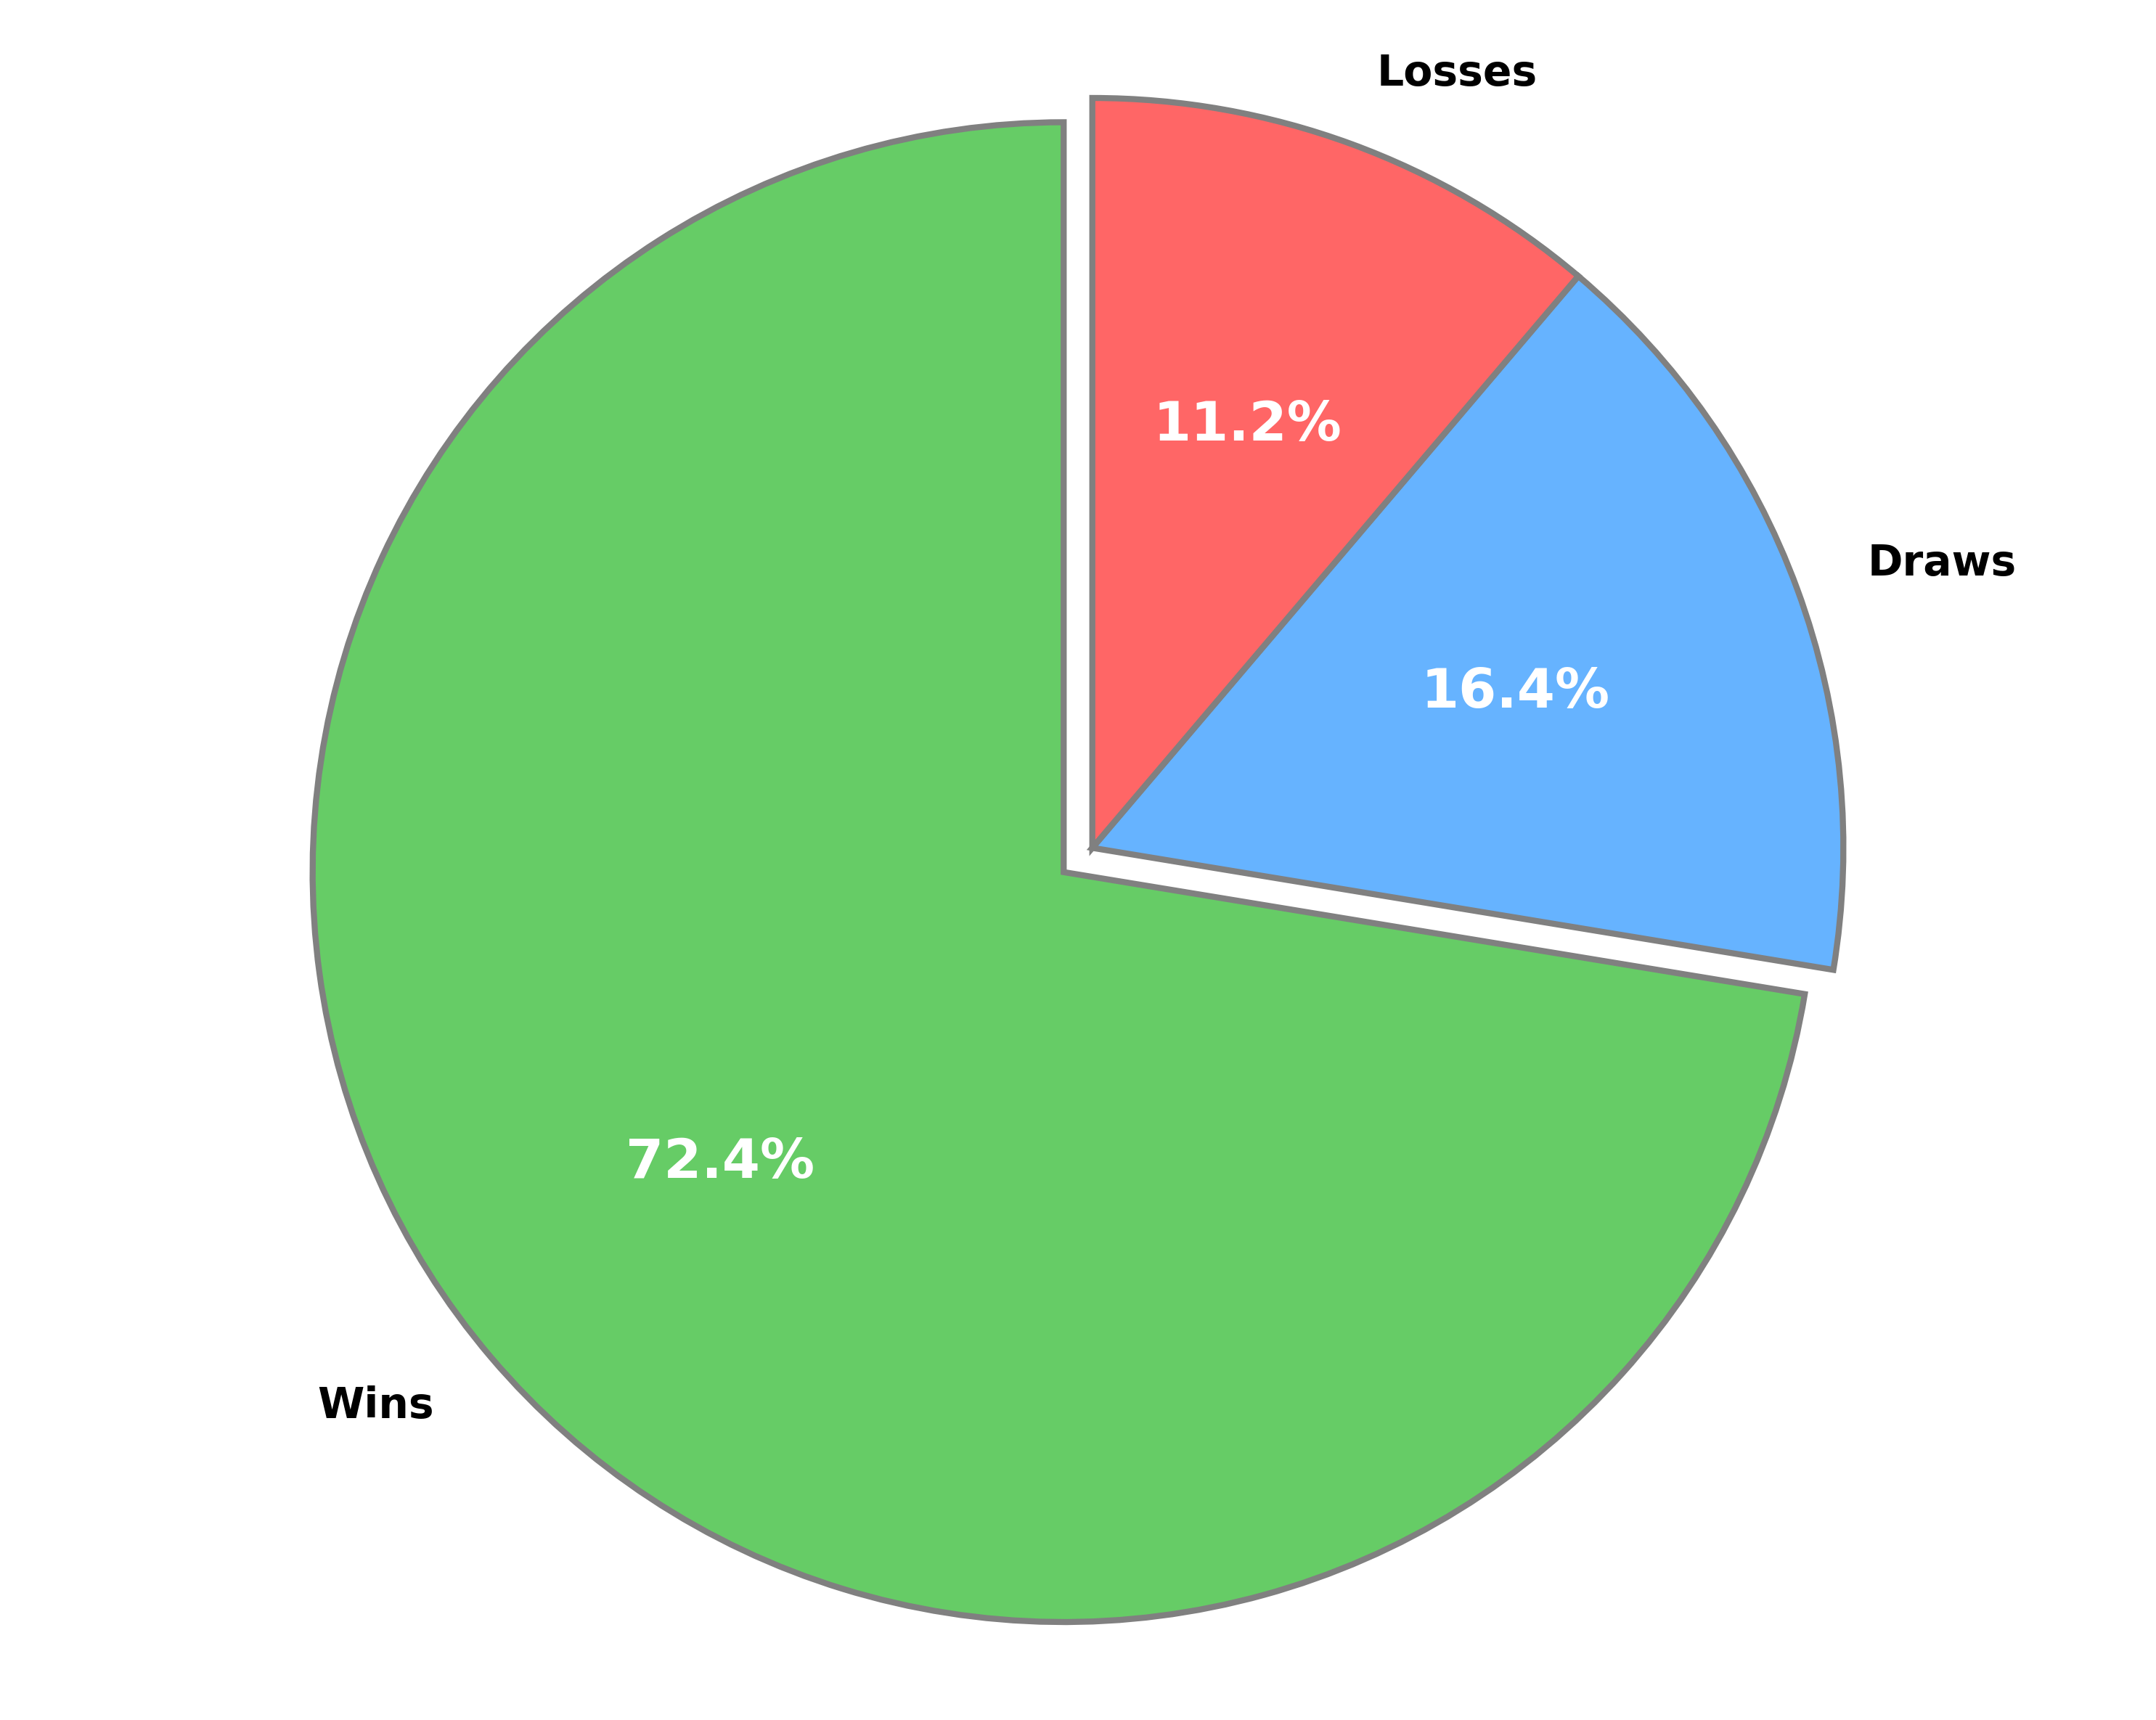
\includegraphics[width=0.4\textwidth]{Plots/winrate_tdmpc.png}\label{fig:wins}}
%    \caption{Performance of the TDMPC agent}
    \label{fig:sidebyside}
\end{figure}

By the conclusion of the 2,000-episode training period, our agent achieves a win rate of approximately 70\% against BasicOpponent-weak (see Figure \ref{fig:wins}). It's worth noting that the training curve had not yet plateaued, indicating potential for further performance improvements with extended training. Due to computational and time constraints, however, we concluded our experiments at the 2,000-episode milestone.

